
%(BEGIN_QUESTION)
% Copyright 2011, Tony R. Kuphaldt, released under the Creative Commons Attribution License (v 1.0)
% This means you may do almost anything with this work of mine, so long as you give me proper credit

Explain the purpose served by conductivity transmitters AIT-341 and AIT-342 in this sour water stripping tower unit (where sulfide-laden water is ``stripped'' of sulfur compounds by the addition of hot steam).:

$$\includegraphics[width=15.5cm]{i0007rx01.eps}$$

Also, calculate the heat exchange rate through exchanger E-9 given a flow indication of 18.5 GPM at FI-98, a temperature indication of 63 degrees F at TG-478, and a temperature indication of 189 degrees F at TG-477:

\vskip 10pt

$dQ \over dt$ = \underbar{\hskip 50pt} BTU/hour

\vfil

\underbar{file i00683}
\eject
%(END_QUESTION)





%(BEGIN_ANSWER)

This is a graded question -- no answers or hints given!

%(END_ANSWER)





%(BEGIN_NOTES)

The purpose of these two conductivity transmitters is to detect heat exchanger leaks.  If a leak allows acidic compounds to enter the cooling water, the water's conductivity value will rise and signal a high alarm.

\vskip 10pt

Cooling water flow rate of 18.5 GPM = 154.32 pounds per minute.  With a temperature rise of 126 degrees F through exchanger E-9 (189 deg F $-$ 63 deg F), this calculates to a heat transfer rate of 19,444.4 BTU/min, or 1,166,665 BTU per hour.

%INDEX% Process: sour water stripping tower (realistic P&ID shown)

%(END_NOTES)


